\chapter{Waveguides}

\section{Introduction}

% EVEREST -> Everest
\begin{figure}[H]
    \centering
    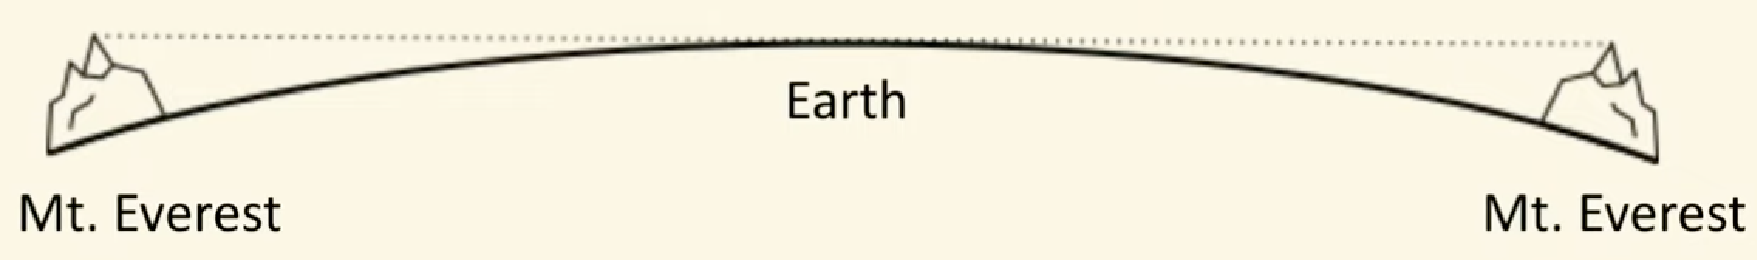
\includegraphics[width=0.9\textwidth]{lesson7/everest.pdf}
    \label{図: 1}
    \caption{The disadvantage of direct transmission of light.}
\end{figure}


00:00
hi and welcome to lesson seven on wave guides
in previous lessons we have talked about how to produce light whether
incoherent or coherent and then we talked about some properties
of coherent light and single photons now we're going to
learn how to make wave guides and what are their basic properties
step one introduction so let's talk about some of the limitations of
unguided light one one of the properties of light is that it travels very fast
which is actually good because if we encode our message
into light then it means that our message will get to the
intended recipient fast also light is fairly unaffected by noise
particularly if it travels in fibers you can pack many fibers together and
they will not be affected by each other's presence
whereas when you compare it to for example copper cables and transmitting

00:01
electrical signals then even the presence of other cables
may interfere with your message also light is now relatively easy to produce
but light travels in straight lines which might sound like a good idea at first
but we will see that actually it's quite limiting in terms of how far
we can communicate so let's consider light traveling in in straight lines
first of course there might be some obstacles between the sender
and the recipient so immediately you uh this will make
it impossible to reach a recipient then it's also actually limited to very
short range either because of the first reason that
you eventually will hit an obstacle but also for the fundamental reason that
earth is curved so let's do some very quick math imagine that this is the
surface of the earth and the curvature of course is uh

00:02
very much exaggerated here and let's say that we've got
two mount everests so that's the highest point
uh on earth and it has a height of just over 8.8 kilometers and let's say that
on this mount everest you place right at the top you place
a light source and you are trying to send it
to a recipient that's standing on top of the other mount everest
so how far can this uh light travel in a straight line
well with some basic trigonometry actually the distance between
mount everest one and two is just 672 kilometers
so even though it seems like we're very far above the earth's surface
we cannot really send the light signal that far and this is discounting
any attenuation coming from the atmosphere so being able to guide or steer light
seems like a very good idea for long distance communication

00:03
so let's see how it all began we can say that it began with john tindall's
experiment in 1870 what he did was he took a big bucket filled with water
and he created a small hole on one side of the bucket at the bottom
and what he noticed was that sunlight that was going into the water
was also exiting through this opening in the bucket
but not only that to his surprise the sunlight followed
the trail that was being taken by the water itself
so the sun sun rays did not just exit the water bucket in a straight line but
they were being guided by the water itself so this was
the third one of the first examples of actual fiber where light was being

00:04
reflected inside the fiber and guided and not traveling just in a straight line
so here's a brief historical outline of uh
the journey that fiber optics have taken so it all began with in 1870
with john tindall's experiment and people were slowly
investigating fiber optics and how to guide light particularly in in glass
but it was only really in 1960 with the invention of laser when people
truly realized the potential of using laser light coupled to fiber optics
so they spent a lot of effort in researching how to do that and in 1966
we people managed to couple lasers with fiber optics
and this really sparked the first information
revolution just to give you some idea how far we've come
in 1970 it was possible to transmit about one percent
of the original light over a distance of one kilometer

00:05
meaning that if you put in light of some power at the beginning after one
kilometer you only had 100th of the original signal
20 years later in 1990 it was possible to transmit 96 of the original power
over the same distance of one kilometer and where are we now in 2021 well
let's have a look at the map of a submarine
fiber optic cables so you can see how many many cables there are connecting
the continents across the pacific across the atlantic
also going from different continents to other continents like this
and this is only the map of the submarine cables
there's a lot more cables going over land
so truly the fiber optic network is the nervous system
of mankind allowing us to communicate within milliseconds
from one side of the earth earth to the other

00:06
so let's have a quick outline of what we're going to talk about in this lesson
first we're going to begin with two basic phenomena of how light behaves
when it hits the interface of two materials
we're going to talk about reflection and refraction
these two are crucial for understanding how fiber optics works
and then we're going to talk about total internal reflection
where we're going to combine reflection and refraction
and derive the condition for total internal reflection total internal refraction
is what we have seen in tyndall's experiment where light was not
escaping the water stream but it was being reflected and guided
by the water stream and then we will conclude by
some basics of fiber optic cables in particular
how they are constructed and what are the differences between various types
of fiber optic cables

\section{Light at an interface}

00:00
step two light at an interface so let's see what happens when a light
is trying to go from one medium into a different medium
before that let's uh see how light can be described
so light can be viewed as a particle traveling in straight lines so basically
like array and in order to describe that we all we
need is geometric optics this is the most
easiest scenario tumor geometric optics relies basically on
the laws of trigonometry to describe how the path of light
changes as it travels from one medium to the other
next step up is if we are interested in the properties of light as a wave
and we've seen uh this with a double slit experiment
that life can light can behave as a wave either
when it's a laser light coherent light or in the form of single photons

00:01
and in order to describe laser light particularly when it's traveling down
a very narrow fibers we need maxwell's equations
and the full theory of electromagnetism this description is a lot harder and
we're not going to use it here and finally the third one
is the description of quantum field theory because light fundamentally is a
quantum field but we're not going to worry about this at all we're only going to
use geometric optics so the most simple description
because mainly we will consider the diameter of the fiber to be much larger
than the wavelength of the light so here d is the diameter of the fiber
and lambda is the wavelength of light and they give you some ballpark of the
of the numbers that we're going to consider
is d varies somewhere bit from 10 all the way up to 200
micrometers whereas the wavelength of light is around
of the order of 1500 nanometers so let's see what happens when the light arrives

00:02
at an interface of two media we're going to consider one medium
usually the air and then some denser medium
let's call it let's say that it's glass and the light ray is going to arrive at
some angle and this angle will always be measured
with respect to the normal to the surface so we're not going to talk about the
angle of incidence as this light as sorry as that angle but the angle
between the light ray and then this orthogonal normal
line to the surface so this is the angle of incidence
and we're going to call it denoted theta i what can happen is that the light can
actually reflect of the surface as this at some angle which we're going to call
theta capital r the angle of reflection and also some portion of the light will
get refracted so it will travel into the medium at some angle theta

00:03
small r the angle of refraction notice that all of these angles are
defined with respect to this dotted line which is the normal
to the surface that's very important and often some portion of the light is
reflected some portion of the light is refracted and actually it gets
transmitted into the other medium in this case we're we're saying that for
example 90 of the light is refracted and enters the glass
whereas 10 percent gets reflected back but we're not going to be too interested
in the relationship of how much gets reflected and how much gets refracted
we are more interested in the angles of reflection and angles of refraction
so what are what is the angle of reflection well that's very simple
the angle of reflection is just the angle of incidence so theta i is equal to

00:04
theta r for example if we keep increasing the angle of incidence so we started
with this light right here but then we consider a different light
ray and then a different one all with different angles of incidence
the corresponding angles of refraction reflection are also increasing
now let's talk about angle of refraction this is going to be a little bit more
complicated as you can see from this image here the angle of incidence and
angle of refraction are different so let's see how we can actually compute them
and for that we need something called refractive indexed of a material
refractive index is defined as follows we're going to denote it as n
and it's given a c over v so n we said is the refractive index c
is the speed of light in vacuum and v is the speed of light in the medium so

00:05
really what refractive index tells us is how much does the speed
of light change in this new medium for example this refractive index of vacuum
is just one why because in vacuum the light travels with the same speed c
so c over c is equal to one air has a slightly larger refractive index but
for our purposes it's basically just one so
the speed of light does not change very much it slows down a little bit
but very very small amount glass on the other hand
has a refractive index of 1.46 so it means that the light travels 1.46 times
slower in the glass than when we compare it with the
speed of light in vacuum and in diamond it travels
even slower by a factor of 2.42 which is the refractive index of diamond

00:06
so let's get back to our example of light ray being incident on a surface
so we're going to denote the refractive index of the top medium as ni
i stands for anything that's incident onto the surface
and nr is the refractive index of the material
into which the light ray transmits and gets refracted
and the angles follow this relationship so the sign of the incident's angle
divided by the speed of light in that medium
is equal to the sine of the refracted angle theta r over the speed of light
in the new medium so we can use we can use this relationship
between the refractive index and the speed of light in the medium
and we just substitute for vi and we substitute for vr and we obtain

00:07
the following relationship it's ni times sin theta i is equal to nr sine theta
r so the refractive index of the medium on top here times the sine of the
incidence angle theta i is equal to the product of the
refractive index of the new medium and times the sine of
angle of refraction and this is known as snell's law
and this law is very useful and we're going to use it extensively
in this and following lessons so before we do any computations let's
see what actually happens uh with the angles as light travels from
let's say a less dense medium into a more dense medium
so what that means is that ni is smaller than nr
for example if we are considering the example of light
going traveling in air and then trying to move into glass again

00:08
substituting into of our snell's law and rearranging a little bit
we've got n i over n r so we brought this n
r on to the other side and then we also divided by
sine theta i so we've got that the fraction of ni over nr
has to be equal to sine theta r over sine
theta i and from our assumption that we are traveling from less than medium into
more dense medium we can see that the fraction of the left-hand side
is smaller than one what this means that this fraction over here
also has to be smaller than one and that's achieved when
theta r is smaller than theta i meaning that the angle of refraction is
smaller than the angle of incidence so we see that when light travels from a
less than medium into more than its medium it bends towards the normal now
what happens in the opposite scenario when we are traveling

00:09
from a mordance medium into a listen's medium well we can go through the same
calculation again but this time we assume that ni is larger than nr
and we substitute it in we see that the ratio on the
left hand side of ni over nr is larger than one
therefore we conclude that the angle of refraction
has to be larger than the angle of incidence so
if we are going from a more than medium into a lessons medium
we are refracting away from the normal

\section{Total internal reflection}

00:00
step 3 total internal reflection in the previous step we have seen that
if light is incident on a surface and traveling from a more than
medium into a less thans medium then it gets
bent away from the normal axis it gets the angle of
refraction so this angle over here is larger than the angle of incidence
so we can have the scenario where we are increasing
steadily the angle of incidence and the refracted beam of light
is being bent further and further away from the normal
axis that's perpendicular to the surface of the material
so can ask the question is there such an angle of incidence
where the refracted beam travels parallel to the surface to the
interface between the two media meaning we are looking for a

00:01
scenario where the angle of refraction is 90 degrees and yes there is
so we are looking for this scenario we have our incident beam
hitting the interface between glass and air at such an angle
such that the refracted beam travels at 90 degrees to the normal
or parallel to the surface between air and glass
so let's now compute this angle using snell's law
we have that the ni the refractive index of glass
times the sine of the angle of incidence is equal to the refractive index
of air and r times the sine of theta r but we know that here we are looking
for a scenario where the sine of theta r is just sine of 90 degrees which
is equal to 1. so we have the following relationship
and we have changed the subscript here on this theta

00:02
to theta c which stands for critical angle
because that's the critical angle where we obtain angle of refraction of 90
degrees now we can just rearrange to get sine
of theta c equal to as a simple fraction of nr over ni in our case here nr
is the refractive index of air and ni is the refractive index of glass
and we can just take the arc sine to obtain
this expression for the critical angle when this happens then we have then we
said that the light ray travels parallel to the
surface but we can also keep increasing the angle of incidence
to fit the eye being larger than the critical angle theta c
and in that case what happens we get total internal reflect
reflection so the light ray comes in and gets totally reflected back to
inside the glass and this is this uh case that we saw in the first step

00:03
uh of tyndall's experiment where the light was being internally reflected and
guided by the stream of water so let's consider some uh numerical examples
here we are keeping the refractive index of the outside medium which for us
is air fixed so it's just 1.00028 it's basically the same as one
and what we are changing is the material of
uh of the fiber so we are changing the refractive index of uh an i
and we are looking at the value of the critical
angle beyond which total internal reflection can occur
so if we are plotting the arc sine of uh
of the previous expression for the theta c then we get the following curve

00:04
so we see that as we are increasing the density of the material we are
decreasing the angle of uh the critical angle beyond which we get total internal
reflection for example if we look at what the interface of water and air
water have refract has a refractive index of 1.33
so that's this line over here and we obtain
a critical angle of around 50 degrees glass is a little bit more dense than
water it has refractive index of 1.46 and the angle of the critical angle
beyond which we get total internal reflection
is a little bit smaller than the water and for diamond which
has a very large refractive index of 2.42 then the angle
is slightly over 20 degrees so what does that
what does all this means that the ang that the critical angle is decreasing
well it means that in class if we want to obtain total internal reflection

00:05
then the angle of incidence which again i remind you is the angle between the
incident light ray and the normal to the surface
has to be large meaning that the angle between the surface
so the measured with respect to the interface between air and glass
has to be quite small then we get total internal reflection
whereas in diamond the light is confined more strongly it can
it can have a incident angle which is smaller than it is in the glass
so it even if it's even if it's incident on the surface at
this much steeper angle it still can get reflected and be contained and guided
by the fiber

\section{Optical fibers}

00:00
step 4 optical fibers let's have a look what a typical optical
fiber consists of on the outer layer we've got the jacket
and this is to protect the inside components of the fiber the next in line
is the buffer now the buffer is there also for protection
but it can also bundle multiple optical fibers
then we've got the cladding over here and this is the material that is
responsible for reflecting um reflecting light back and keeping it
contained within the inside which is the core also cladding
serves as a form of protection and prevents crosstalk because if you have
two uh cores next to each other then light can easily escape to the other core
so you must separate them somehow and that's the purpose of the cladding

00:01
so these two components are the ones that are optically
important parts core is the one that carries the light signal
and it has some refractive index and c whereas sorry nf for uh nf for fiber
whereas cladding has a smaller refractive index nc and that's the one that is
responsible for uh reflecting light back into the core and
keeping it constant inside the fiber and there are two main types of fibers one
is the multimode fiber over here so you can see that
here the modes are represented by different spatial
beams bouncing inside the fiber and single mode fibers which are so narrow
that there's only one mode permitted to travel inside the fiber

00:02
so let's look at multi-mode fibers first as we said here all of these rays they
represent various modes of light traveling inside the fiber
and what's important for multi-mode fibers is the angle of acceptance
this is the angle represented by this gray cone over here and if the light
comes traveling inside the fiber within this light cone
then it will couple to the fiber and undergo
many internal reflections inside the fiber
and basically be carried inside and be guided by the fiber
but if the incident angle of the light is such that it is outside
of the acceptance cone then it will just hit the cladding and get refracted
outside and get absorbed so it will not be coupled to the fiber
so let's apply snails law and actually calculate what is the maximum permissible
permitted angle such that we couple to the fiber

00:03
so we have the following scenario in here we actually have
two interfaces one interface is the usual
between the fiber with refractive index and f
and the cladding with refractive index and c but now we also have to consider
the light coming into the fiber so we also consider refractive index of
some material that's outside of the fiber and we will denote it by ni and we've
got these three angles we are looking for the maximum
theta maximum permitted angle and if we multiply it by two this is called
the acceptance angle and we want this angle to be such that
when the light gets refracted into the fiber and then hits the cladding it gets
reflected completely and totally back into
inside the fiber so this angle we set to theta c
which is the critical angle needed for total internal reflection

00:04
using basic trigonometry then we know that this
angle of refraction at the surface of the fiber
and whatever material is outside of the fiber has to be 90 degrees minus theta c
and we all know from previous step that if we take the sine
of this critical angle so this angle over here
it has to be equal to the ratio of the refractive indices
of the cladding and the fiber so sine theta c is equal to nc over nf
then we continue using our snell's law so
at this interface between the fiber and the outside material
we write that ni the refractive index of the outside material
times sine theta max has to be equal to the refractive index of the fiber times
sine 90 degrees minus theta c which is the angle of refraction
over here measured with respect to the normal of the surface

00:05
which in this case is given by this horizontal dashed line
and we can simplify using trigonometric identity sine
90 degrees minus theta c is just equal to the cosine of that angle
theta c and we can use another trigonometric identity where we use the fact that
sine squared of an angle plus the cosine squared of the angle
has to be equal to one so cosine of theta c is just equal to
1 minus sine squared theta c the whole expression square rooted and using
the expression that we have over here for the critical angle
we can just substitute an expression for sine
sine squared theta c which is just nc squared over nf squared so
finally we have the following expression multiplying
this by nf we get that the ni times sine theta max is equal to the

00:06
square root of nf squared minus nc squared and this gives us the theta max the
maximum angle of acceptance and therefore also the cone of acceptance
and this number on the left hand side this product of the refractive index
times the max sine of the maximum acceptance angle is known as
numerical aperture and the higher the numerical aperture is
the better we can couple to the fiber meaning that this
incident angle over here which we are calling theta max is allowed to be larger
so let what are some properties of multi-mode fibers
well we said that their diameter is much larger
than the wavelength of the light and typically they've got
diameters larger than 10 micrometers and they can go up to something like 200
micrometers so we said in order to describe their
behavior it is enough to consider light traveling as a

00:07
as a particle traveling in straight lines and using basic trigonometry
so we can use geometric optics which we have been doing so far
in order to derive some useful properties of the multimode fiber
second the light inside travels at different angles meaning that it can
carry multiple modes at the same time but what this causes is because the path
lengths of the various parts of the various light rays
differ we get mode dispersion and we will describe that in a later lesson and
look at it more closely and such a fiber because of mode dispersion is
more suited for short distances so meaning inside office networks or
campus networks and also it is relatively cheap to manufacture
mainly because it's quite thick on the other hand a single mode fiber
can carry only a single mode of light so there's only one ray traveling at it

00:08
in one direction like this and now the diameter is uh typically smaller
than 10 micrometers and just to give you an idea how thin that is
the human hair is usually larger than 20
micrometers there's a large variance but it's between
20 and perhaps 200 micrometers so they're extremely extremely thin
and because they are so thin it is no longer possible to describe them as using
geometric optics we have to resort to using electromagnetic
theory and maxwell's equations but because they are so thin and there's
only a single mode there is no mode dispersion
and that is why they allow for very high rate of transfer of data and therefore
they are suitable for long distance communications
they have to be boosted by repeaters approximately every 50 kilometers

00:09
but we will see how that can be achieved in a later lesson
but because they are so thin they are quite expensive to produce
and a small small note at the end the first transatlantic fiber optic cable
which was called t8 was laid in 1988 between tuckerton new jersey
and then it traveled uh across the atlantic and then split
into the uk and france and it was um constructed at a cost of approximately 335
million us dollars and it was retired in 2002.
so it was predicted that the bandwidth of this fiber optic cable would last for
a long time and perhaps never be reached the bandwidth was 280 megabits per
second which can carry around 40 000 phone circuits simultaneously

00:10
and this capacity was reached in 18 months
now this just demonstrates how quickly how quickly we can consume data and how
quickly we need to transfer data and the size of
the data that we need to transfer


\newpage
\begin{exercises}
\exer{Consider the following quantum state:}
\begin{equation*}
\ket{\psi} = \frac{\sqrt{3}}{2}\ket{0} + \frac{1}{2}\ket{1}
\end{equation*}
\subexer{Find the probability of measuring a zero.}
\subexer{Find the probability of measuring a one.}


\end{exercises}

\newpage
\section{Quiz}

\section{Further reading Lessons 5-7}

Lesson 5

This Lesson discusses the various types of light depending on their coherence properties. Coherent light produced by lasers is crucially important from the perspective of communication. A good qualitative as well as quantitative introduction to lasers can be found in Chapter 1 of:

Orazio Svelto, Principles of Lasers, Springer, 2009.

A great discussion of lasing behaviour from the perspective of a mathematician (but still explained very intuitively) is in Chapter 3 of the classic:

Steven H. Strogatz, Nonlinear Dynamics and Chaos: With Applications to Physics, Biology, Chemistry, and Engineering, CRC Press, 2000.

Lesson 6

Two great optics textbooks for this Block as well as the following ones are:

Eugene Hecht, Optics, Pearson, 2015.
Grant R. Fowles, Introduction to Modern Optics, Dover Publications, 1989.
Bahaa E. A. Saleh, Malvin C. Twitch, Fundamentals of Photonics, Wiley-Interscience, 2007.

These books focus on wave and geometric optics and provide a good foundation for transitioning to quantum optics which we will do later.

Interference is an extremely important concept we encourage you to read and understand the discussion in Chapter 1 in:

Richard P. Feynman, Robert P. Leighton, Matthew Sands, The Feynman Lectures on Physics, Vol. 3, Addison Wesley, 1971.

Lesson 7

This Lesson relies mainly on the geometric description of light propagation. Section 4.3 and Section 5.6 of Hecht’s textbook contain great discussion of reflection and propagation in optical fibers, respectively.
